\documentclass{beamer}
\usepackage{xmpmulti}
\usepackage{caption}
\usepackage{subcaption}
\usepackage{epstopdf}
\usepackage{graphics}
\usepackage[pdftex]{graphicx}
\usepackage{tikz}
\usepackage{amsmath}
\usepackage{verbatim}
\usepackage{color}
\usepackage{natbib}
\usepackage{bibentry}
\bibliographystyle{apalike}
\usepackage{chngcntr}
\usepackage{color}
\usepackage[subnum]{cases}
\usepackage{wrapfig}
\definecolor{links}{HTML}{2A1B81}
\hypersetup{colorlinks,linkcolor=blue,urlcolor=links}
\setbeamertemplate{navigation symbols}{}
\usepackage{caption}

\captionsetup[figure]{labelformat=empty}

\usetheme{Montpellier}
%\setbeameroption{show notes}
\beamersetuncovermixins{\opaqueness<1>{25}}{\opaqueness<2->{15}}

\date{\today}

\begin{document}


\title{Cognitive Ecology: Systemic Complexity and Cognitive Diversity.}
%Here's how I can see your paper:
%A) motivation of big project: aggregation of diverse beliefs. Want to measure relationship of diverse beliefs to performance
%B) This paper: describing causal beliefs and measuring diversity
%C) In math, define a causal belief structure, and relate it to a probability density function
%D) In math, show how the Weitzman measure + the JS metric yield a measure of the diversity of probability density functions.
%E) In a simulation, describe 5 macroeconomic variables, create say 10 causal belief structures out of them.
%F) Specify the resulting probability density functions. Calculate diversity.
%G) Show that as you change how you create the 10 causal belief structures, the diversity measure changes in a plausible way.
%H)Conclude.



\author{Johannes Castner}
\institute{Columbia University}
\begin{frame}
\titlepage


\end{frame}

%\frame{\frametitle{Table of contents}\tableofcontents}

\begin{frame}
%\frametitle{Basic Claim}
%With Rational Inattention (RI) and particular plausable mental representations, the more complex the system is in which attention is allocated, the more diverse will be the opinions about the system's mechanics. \\
\\
\begin{figure}
  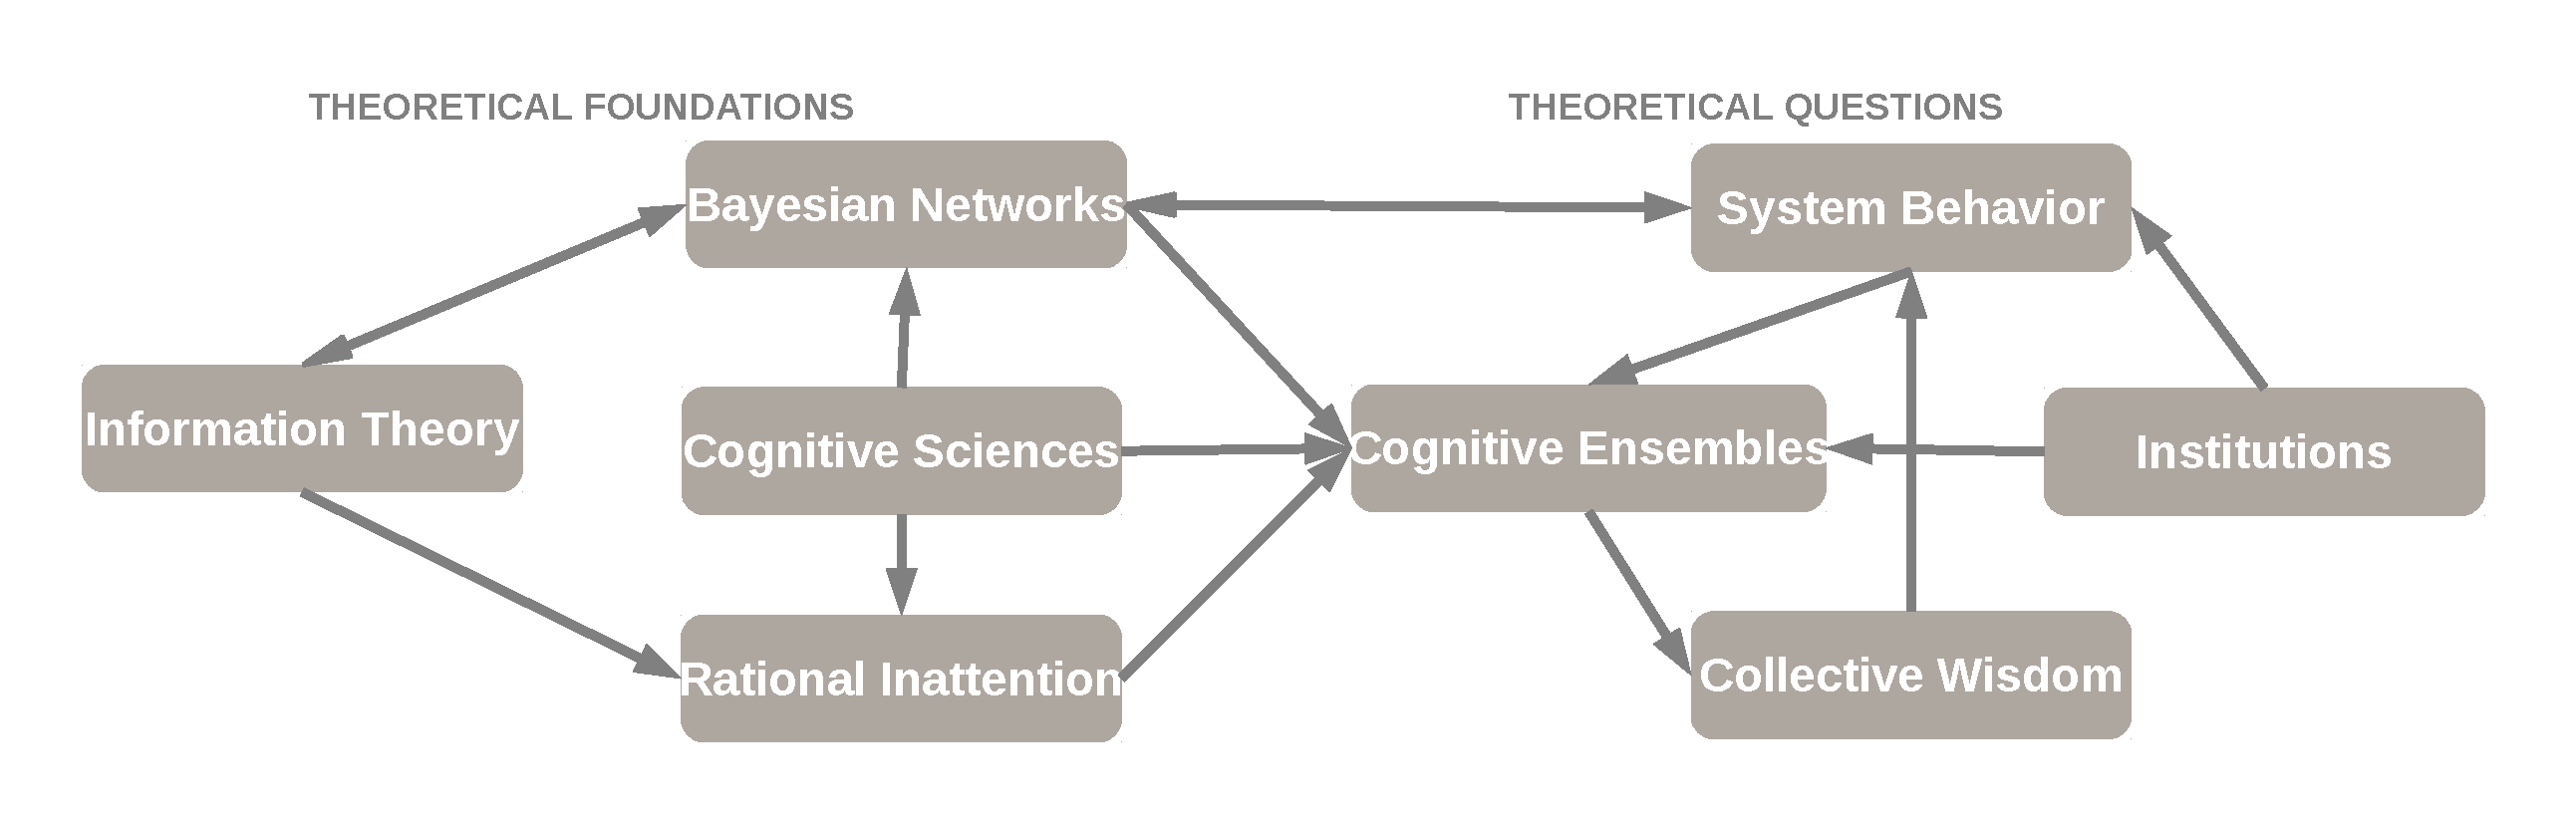
\includegraphics[width=\textwidth]{FoundationsQuestions.pdf}
\end{figure}%
%Hypothesis: the more complex the system, the more diverse the beliefs.
\\
%A principled account of how the limits of human cognitive processing interact with the properties of the systems that form the content of beliefs, to give rise to Cognitive Diversity.
\\
\end{frame}
\begin{frame}
\begin{itemize}
\item[RI] Rational Inattention is an economic theory that takes as a premisse that attention is a scarce resource \citep{Woodford12}.

\item[IT] Information Theory \citep{CoverThomas} equips this theory with theoretical limits on information processing capacity, given some noisy channel: here a model for human visual perception.
\end{itemize}       

RI, equipped with channel capacity makes clear and successful predictions of individual perception: peoples' perceptions should be accurate for most of the data, but should be error prone for rare states of the system.
\\

I use this perceptual theory to derive implications for the diversity of beliefs in cognitive essembles, such as markets and political systems: The amount of bias should be the same for all individuals if cognitive costs are the same, but in low probability states of the system the actual long-term biases can be quite different with slightly different priors, even if the same observations were made. 
\end{frame}     
\begin{frame}
\begin{itemize}
\item[BN] Bayesian Networks are types of Probabilistic Graphs \citep{Koller03}, which use the concept of causation \citep{Verma90} as an efficient construct for humans to accurately estimate high dimensional joint-distributions with a small number of parameters \citep{Griffith08}.
\end{itemize}
%Diversity of beliefs then interact with assymetries in budget constraints for pessimists and optimists to bring on bubbles.     
\end{frame}
\begin{frame}
\frametitle{Michael Woodford's of Rational Inattention}
\citet{Sims98, Sims03, Sims11} proposes a general theory of the optimal allocation of limited attention: 
\begin{itemize}
\item there is a ``true state'', $x$ and 
\item a mental representation, $r$
\end{itemize} 
In my case $x$ represents vector realizations of a set of binary variables and $r$ is a set of parameters and relations, describing a subjective probability distribution over $x$ (more on that soon). 
\end{frame}
\begin{frame}
\frametitle{Sims's Hypothesis of Rational Inattention}
RI hypothesis:
Representation $r$ and conditional probabilities $\{p(r|x)\}$ maximize performance (the expected number of correct decisions), subject to an upper bound on the information that the representation conveys about the state:

\begin{equation}
I_{xr}=E_{x, y}\left[ \log{\frac{Pr(r|x)}{Pr(r)}}\right]
\end{equation} 

This quantity is Shannon's 1948 measure of mutual information. 
\end{frame}
\begin{frame}
 Decision makers then maximize:
\begin{equation}
\Pi(x, r) - \theta I_{xr}, 
\end{equation} 
where $\Pi(x, r)$ is some objective function and $\theta > 0$ is a unit cost of information-processing capacity.
\\

If the system that generates observations, $x$, becomes more complex, each single representation should convey less information about $x$ and a greater variety of representations should appear in a population of capacity constrained individuals. \\
\\

The more complex the system, the more features among which to allocate attention.    
\end{frame}

\section{Measuring Mental Models (Bayes Nets)}
\begin{frame}
\frametitle{Mental Models}
According to \citet{Tenenbaum2011} 
\begin{quote}
We [humans] build rich causal models, make strong generalizations, and construct powerful abstractions, whereas the input data are sparse, noisy, and ambiguous--in every way far too limited. A massive mismatch looms between the information coming in through our senses and the outputs of cognition.
\end{quote}
\end{frame}
\begin{frame}
\frametitle{Probabilistic Graphs as Efficient Mental Representations}
\begin{figure}
  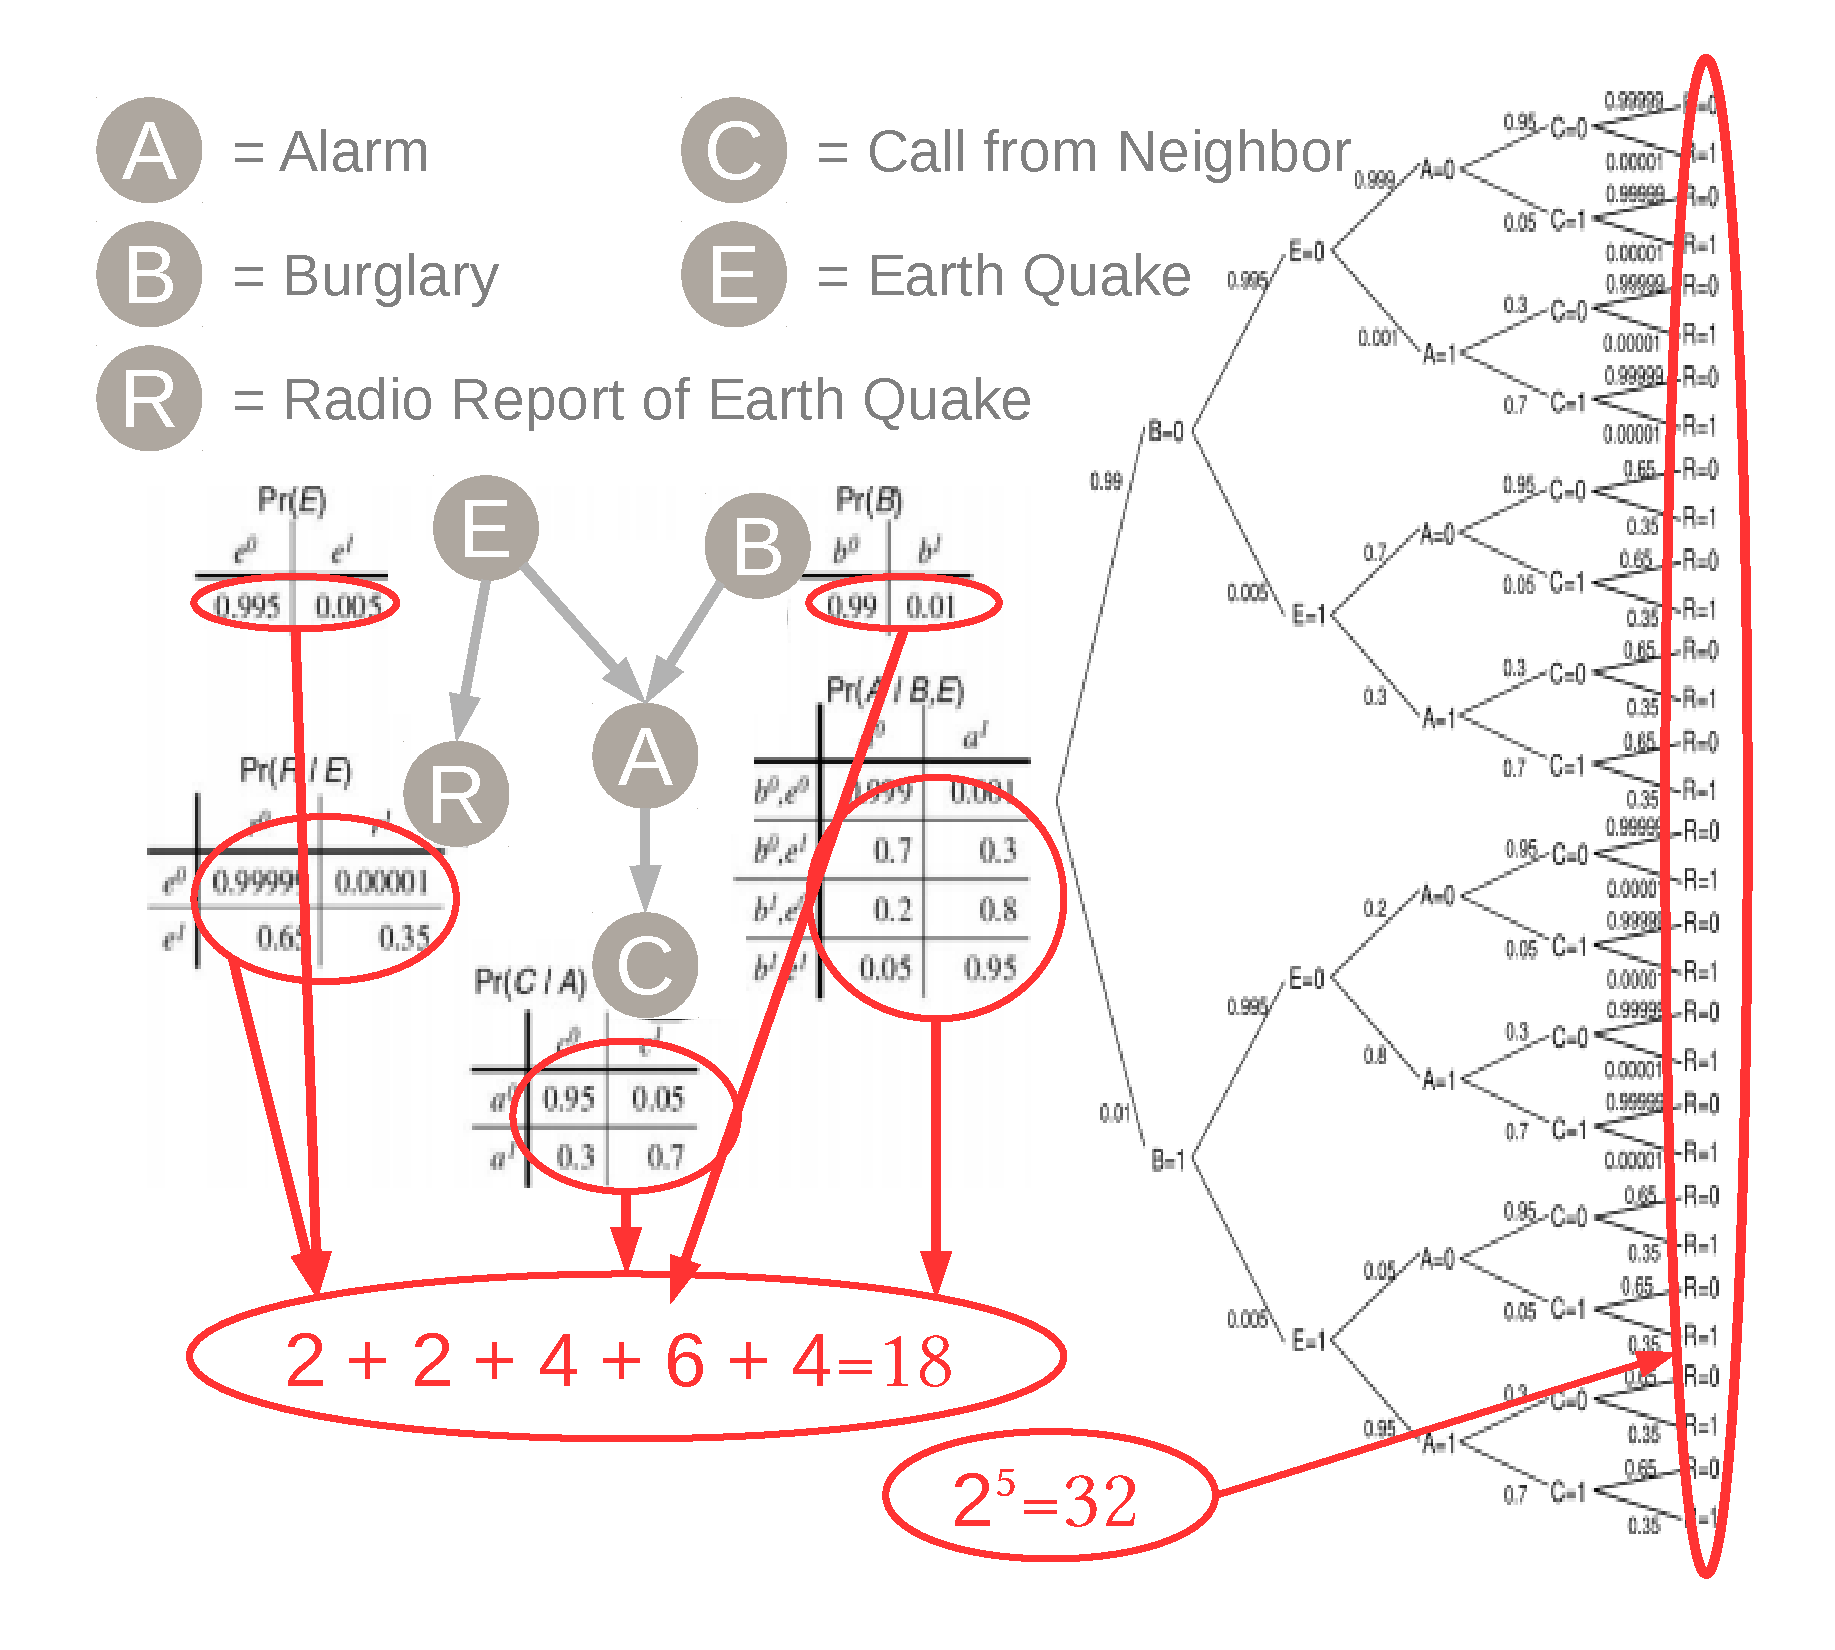
\includegraphics[width=0.7\textwidth]{ParameterExplosion.pdf}
\end{figure}
\end{frame}
\begin{frame}
\frametitle{Measuring the Diversity of Representations}
A well-known measure of distance between two distributions, $P$, $Q$ is the Kullback–Leibler Divergence
\begin{equation}
D_{KL}(P || Q)=\sum_i P(i)\log\left(\frac{P(i)}{Q(i)}\right)
\end{equation}
of which the Mutual Information $I_{xr}$ -- used in the Rational Inattension literature -- is a special case.
\\

$D_{KL}(P || Q)$ has serious flaws as a measure of distance: it is assymetric and unbounded. 
\\

The principled solution is the Jensen Shannon Divergence, the square root of which is a metric:
\begin{equation}
D_{JS}(P || Q)= \lambda D_{KL}(P || M) + (1-\lambda) D_{KL}(Q || M), 
\end{equation}
where $M = \lambda P + (1-\lambda)Q$ and where usually $\lambda=\frac{1}{2}$.     
\end{frame} 
\begin{frame}
\frametitle{The N-Point Jensen Shannon Divergence and Diversity}
The Extension to the two model comparison of distributions $Q$ and $P$ is a measure of how much information there is in an average one bit draw from one of $N$ distributions, $P_1, \ldots, P_N$. This is called the $N$-Point Jensen Shannon Divergence:
\begin{equation}
JSD_{\pi_1, \ldots, \pi_N}(P_1, \ldots, P_N)=H\left(\sum_i\pi_iP_i\right)-\sum_i \pi_iH(P_i),
\end{equation} 
where $H(\cdot)$ is the Shannon Entropy. Deviding by $\log_2(N)$ and taking the square root, I get my desired Cognitive Diversity measure
 \begin{equation}
Diversity(P_1, \ldots, P_N)=\sqrt\left(\frac{JSD_{\pi_i=\frac{1}{N}; \forall i}(P_1, \ldots, P_N)}{log_2(N)}\right)
\end{equation} 
\end{frame}
\begin{frame}
The question then boils down to the following: Does individual optimizing of $\Pi(x, r) - \theta I_{xr}$ in more complex information environments lead to more diverse solutions than in less complex information environments, where the diversity of representations is measures as
\begin{equation}
Diversity(P_1, \ldots, P_N)=\sqrt\left(\frac{JSD_{\pi_i=\frac{1}{N}; \forall i}(P_1, \ldots, P_N)}{log_2(N)}\right)
\end{equation}

Theoretically, I want to work this out more fully and for asking this question empirically I have built a special experimental platform, which I will discuss next.   
\end{frame}
\begin{frame}
\small
\begin{figure}
\frametitle{A Cognitive Economics Experiment}
A participant's goal: (for example) predict Interest Rates. 
        \centering
        \begin{subfigure}[b]{0.5\textwidth}
                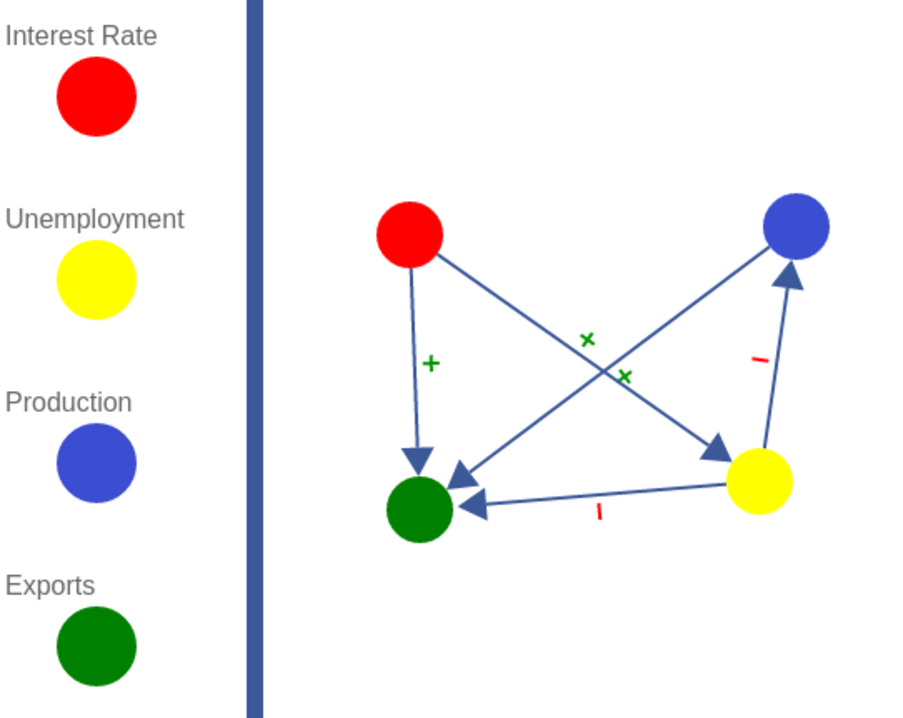
\includegraphics[width=\textwidth]{Complex.pdf}
                
        \end{subfigure}%
       \caption{A belief system about a financial system: The nodes are variables and the arrows are causal relations.}
\end{figure}
\end{frame}

\begin{frame}
\begin{figure}
        \centering
        \begin{subfigure}[b]{0.3\textwidth}
                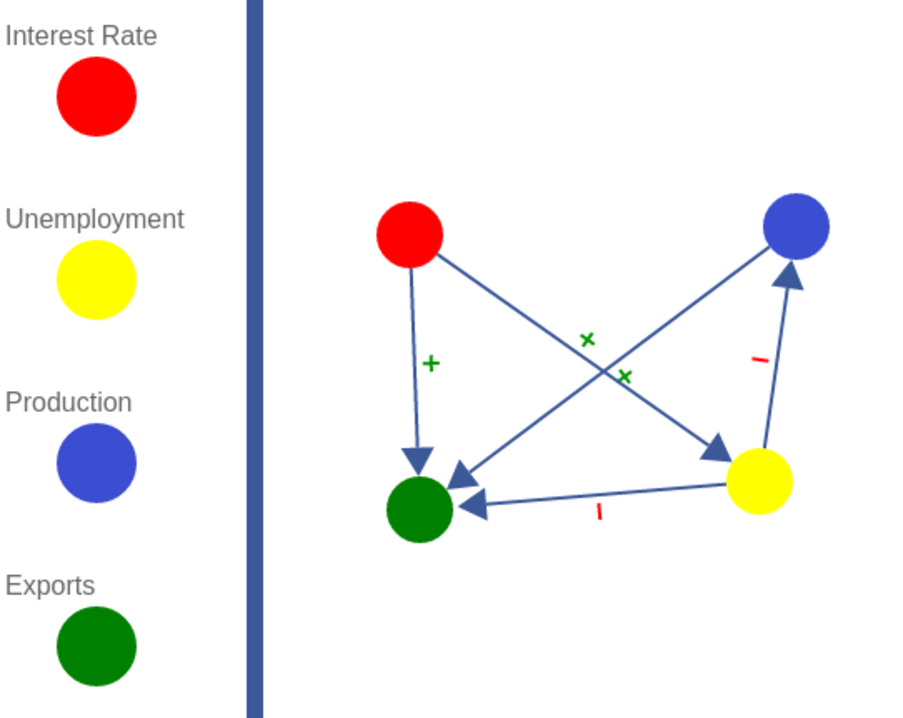
\includegraphics[width=\textwidth]{Complex.pdf}
                
        \end{subfigure}%
       \begin{subfigure}[b]{0.7\textwidth}
        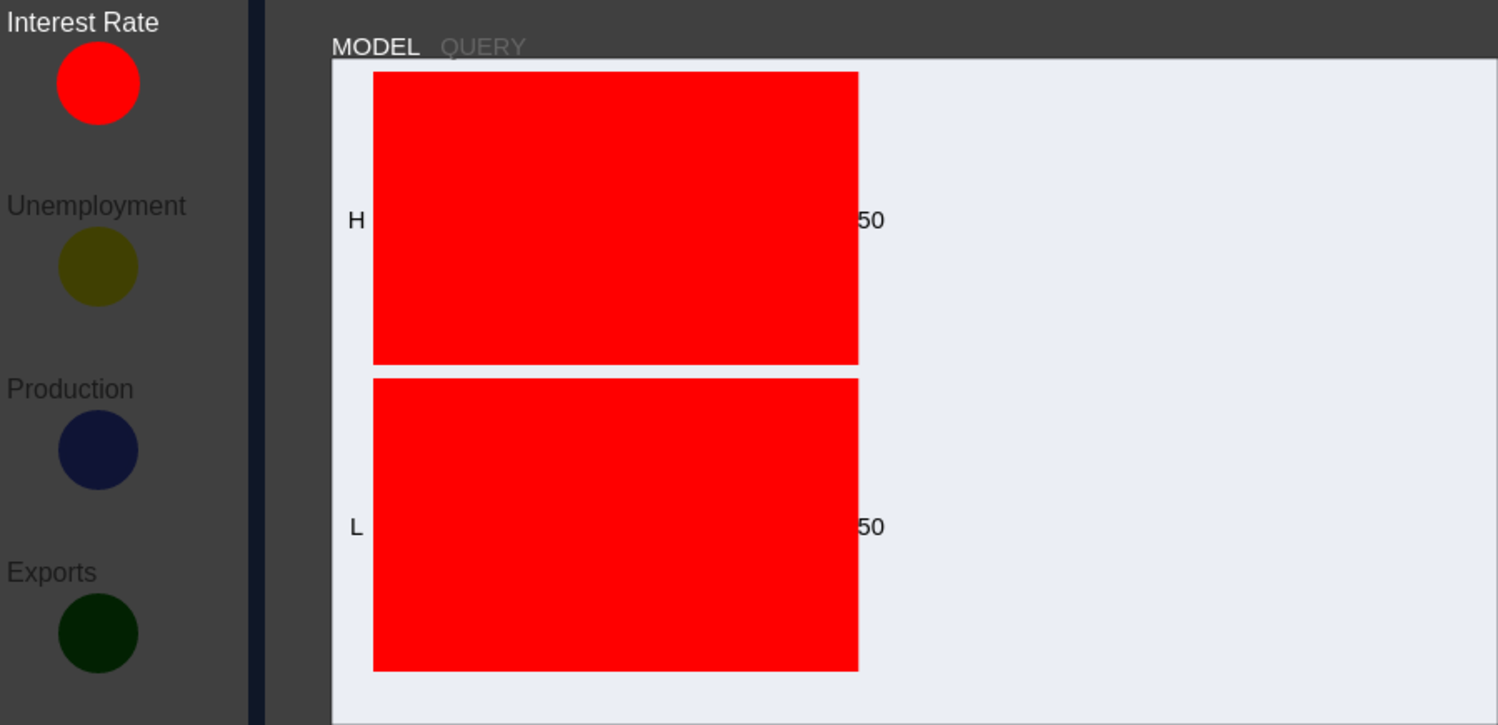
\includegraphics[width=\textwidth]{UncondParams.pdf}
       \end{subfigure}%       
\caption{Each variable here can take on two values: ``H'' (for High) and ``L'' for Low.}
\end{figure}
\end{frame}

\begin{frame}
\begin{figure}
        \centering
        \begin{subfigure}[b]{0.3\textwidth}
                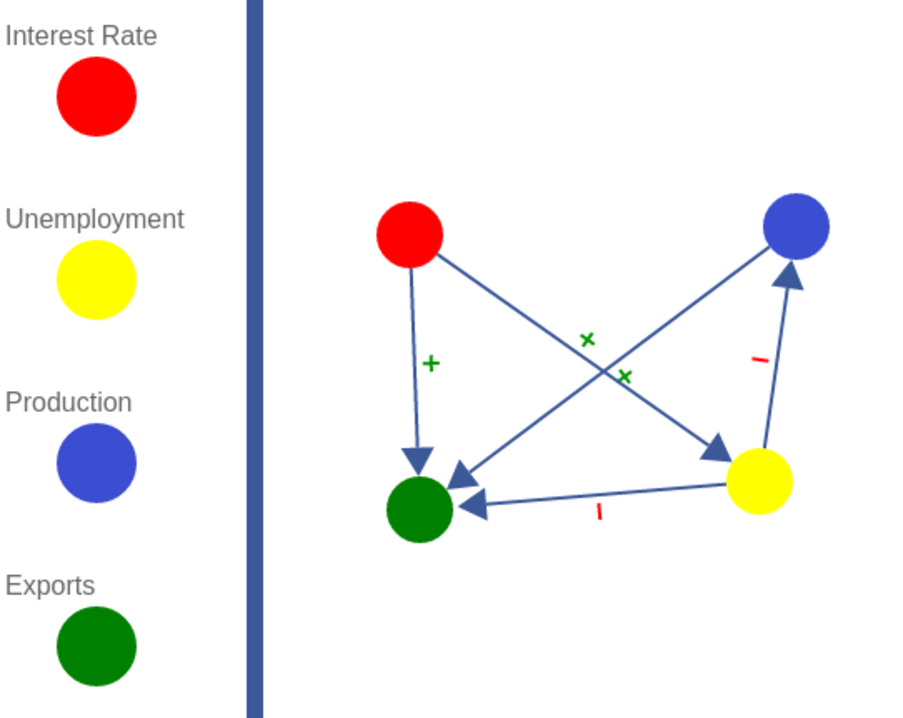
\includegraphics[width=\textwidth]{Complex.pdf}
                
        \end{subfigure}%
       \begin{subfigure}[b]{0.7\textwidth}
        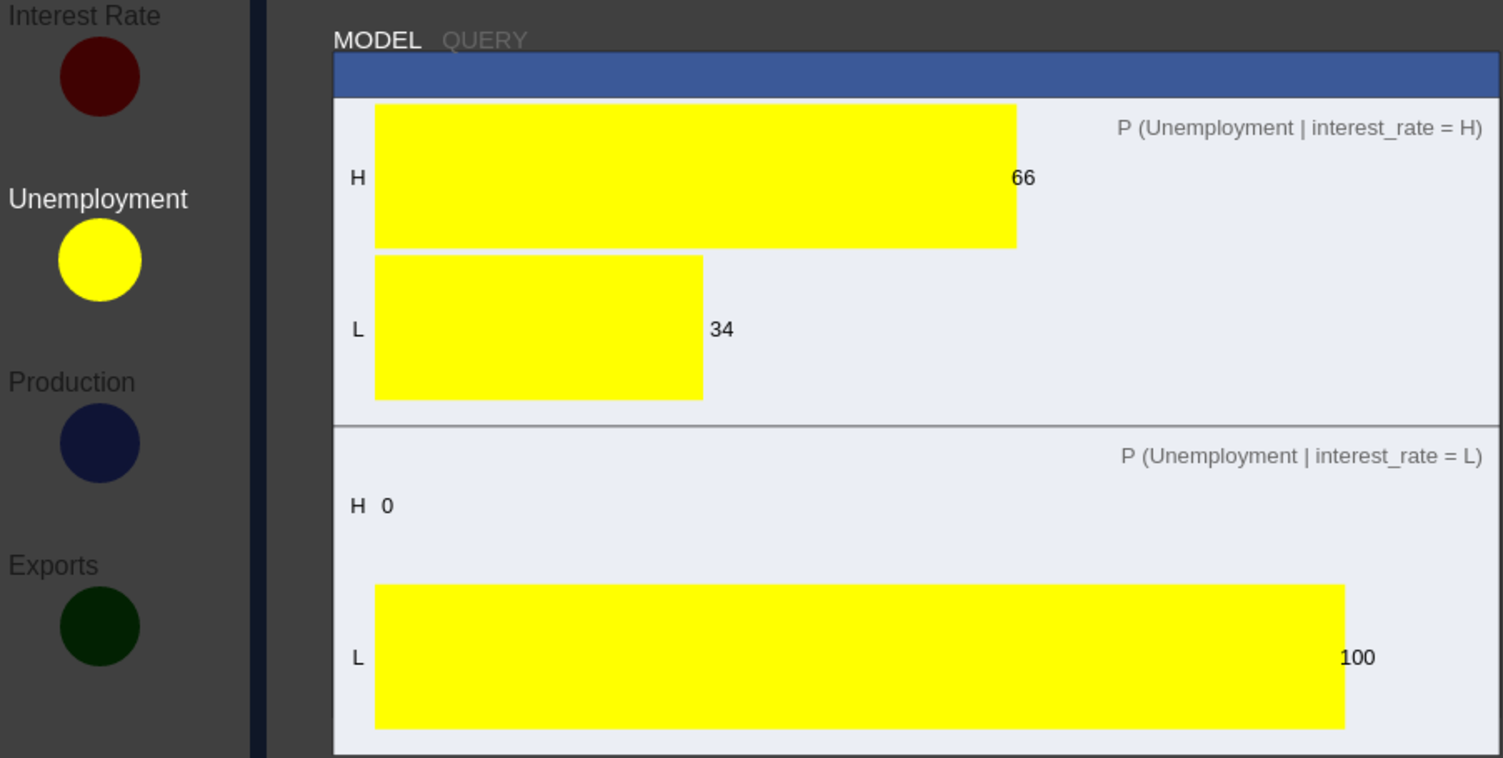
\includegraphics[width=\textwidth]{SettingParameters.pdf}
       \end{subfigure}%       
                \caption{Conditional Probability Model.}
\end{figure}
\end{frame}

\begin{frame}
\begin{figure}
        \centering
        \begin{subfigure}[b]{0.3\textwidth}
                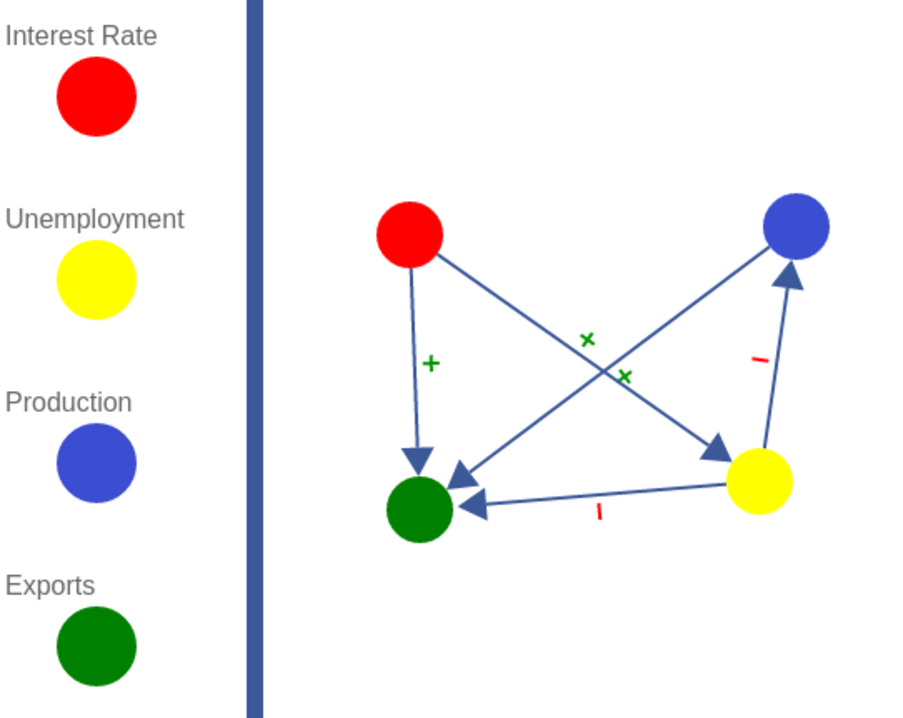
\includegraphics[width=\textwidth]{Complex.pdf}
                
        \end{subfigure}%
       \begin{subfigure}[b]{0.7\textwidth}
        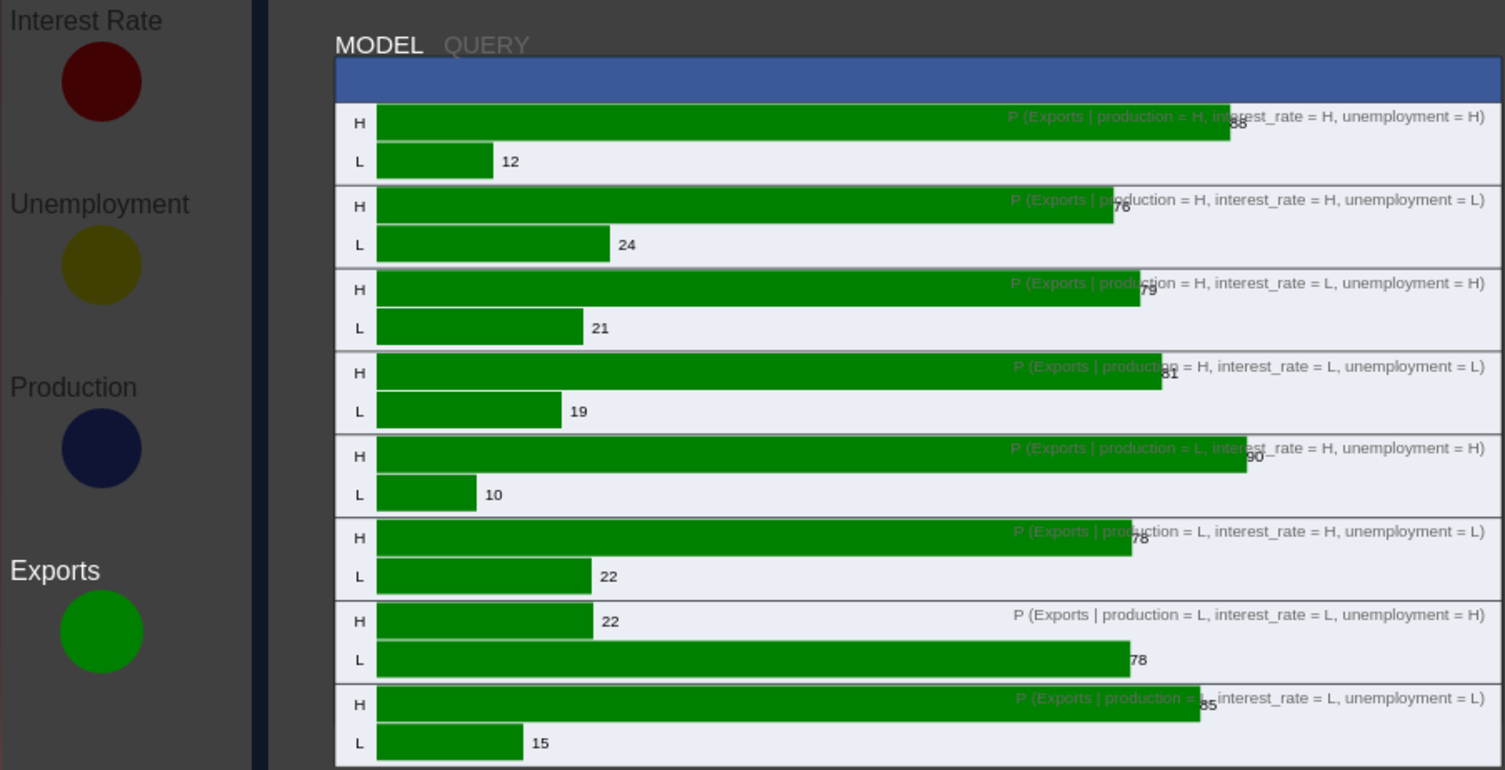
\includegraphics[width=\textwidth]{ManyParams.pdf}
        \end{subfigure}%       
                \caption{Conditional Probability Model with many parent nodes.} 
\end{figure}
\end{frame}

\begin{frame}
\frametitle{Simple and Complex}
\begin{figure}
        \centering
       \begin{subfigure}{0.4\textwidth}
        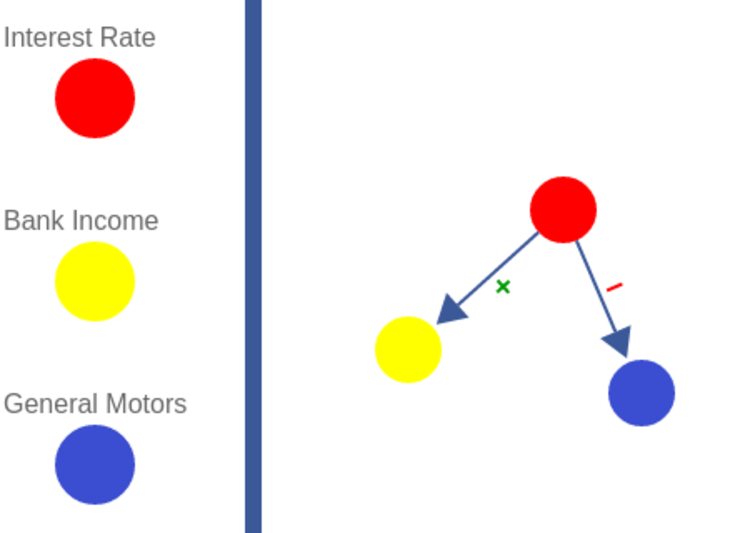
\includegraphics[width=\textwidth]{SimpleModel.pdf}
                         \end{subfigure}
\begin{subfigure}{0.4\textwidth}
        \includegraphics[width=\textwidth]{ComplexModel.pdf}
                %\caption{The Complex Case.}
        \end{subfigure}%    

\end{figure}
\end{frame}



\section{The Experiment} 
\begin{frame}
\frametitle{The Experiment}
Today's experiment is a trading and thinking game.
\hfill \break
At the beginning of this game you will be given
``points'' and ``shares''. The relative amounts of points
and shares may be different from person to person.
In each period you can build a model of how you think
things work (how things affect each other) and then
buy shares from and sell shares to a computer with ``random beliefs'', which means that the computer randomly draws a ``model'' of the system and will accept and reject offers from you accordingly.
%\hfill \break
There will be a total of 12 periods. In the first period,
you will have five minutes to build a model of how
you think things are related. Then there will be five
two minute periods of trading. Next, you will be given
another five minutes to adjust your model, followed
by another five two minute trading periods.
 
\end{frame}
\begin{frame}
Each share pays 100 points if the ``betting'' variable
takes on the value ``H'' at the end of that period;
otherwise it pays out 0 points. The ``betting'' variable is drawn at random in each period from the list of variables visible as colored circles on the left side of your screen. 
\hfill \break
The realization of any variable (``H'', ``L'') may depend on the concurrent values of other variables, but is independent from period to period. There are no causal cycles and models with cycles are not allowed. 
At the end of each period, all earned points are added to
your total score. Then, all shares expire worthlessly and you
are given new shares and points to use in ``betting'' against the machine.
\end{frame}
\begin{frame}
\frametitle{Example}
Suppose that the Interest Rate is our current betting variable and that the value of the Interest Rate is ``H'' at the end of some period. Further, suppose
that you have 5 shares and 150 points at the end of that same period. Then 5*100 +150=650 points are added to your
total score. If the interest rate takes on the value ``L''
instead, only 5*0 + 150 = 150 points are added.
\begin{figure}
        \centering
        \begin{subfigure}[b]{0.5\textwidth}
                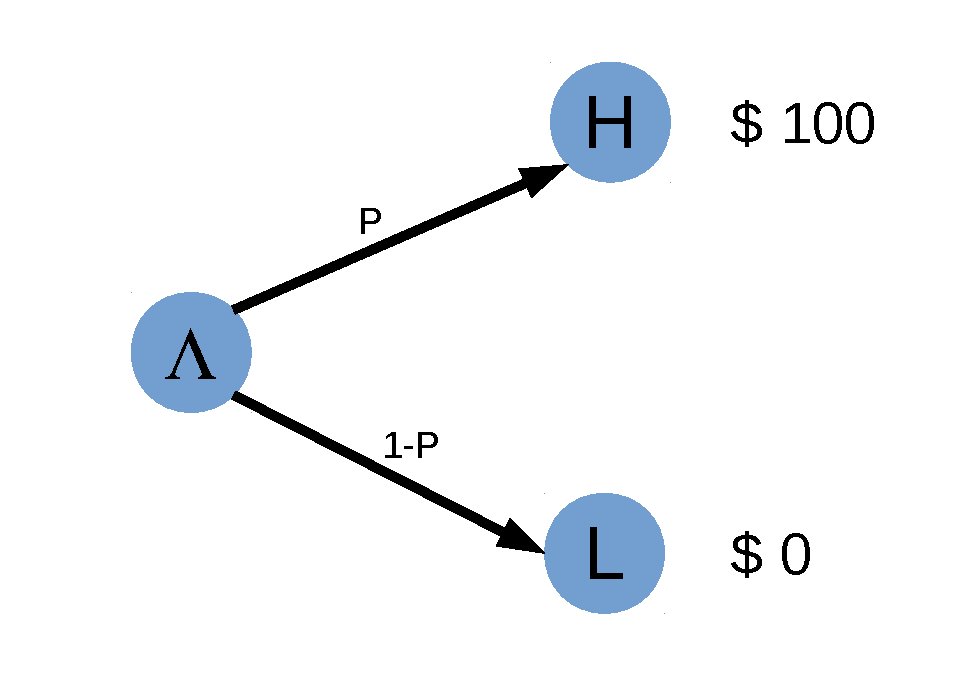
\includegraphics[width=\textwidth]{SimpleLottery.pdf}
                
        \end{subfigure}%
       \caption{If ``H'' occurs, a person holding $X$ shares of this lottery will win X*100 points; otherwise 0 points.}
       \label{fig:alarm}
\end{figure}
\end{frame}
\begin{frame}
\begin{figure}
        \centering
        \begin{subfigure}[b]{0.5\textwidth}
                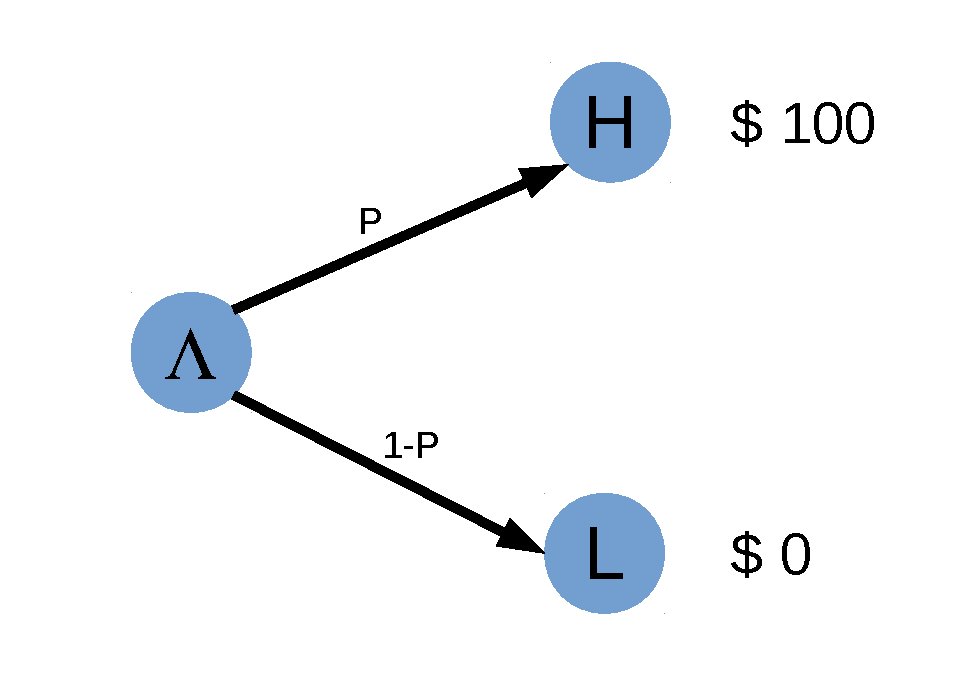
\includegraphics[width=\textwidth]{SimpleLottery.pdf}
                
        \end{subfigure}%
       \caption{If ``H'' occurs, a person holding $X$ shares of this lottery will win X*100 points; otherwise 0 points.}
       \label{fig:alarm}
\end{figure}
It is your job to determine what $P$ is in the above lottery, based on the values taken on by the other variables.  You also will observe a ``history'' of past runs. Each run is independent of the others and the concurrent influence between the variables does NOT change over time. 
\hfill \break
\end{frame}

\begin{frame}
\frametitle{Earnings}
In this game, there exists a true model that generates the data, which is of the same type as you are constructing and in principle it is possible for you to reconstruct the true model. 

Your earnings in this game will depend on your performance and randomness coming from two sources: 
\begin{enumerate}
\item the randomness in the true model that generates the observations you seek to explain and
\item the beliefs about this randomness as drawn by your computer opponent 
\end{enumerate}
The average player will earn $\$12.50$. However depending on your modeling skills and on luck, your earnings may be substantially higher or lower. 
\end{frame}
\begin{frame}
\frametitle{Earnings}
In the game, you can keep track of your points. The higher those are the more you will earn, the exact exchange rate between your points and dollars is determined by the total amount of points that are earned (the group of 20 people is to share a dollar price of $\$250$), so that
\begin{equation}
 250 * \frac{\mbox{your points}}{\mbox{total points of all twenty players}} = \mbox{your dollar earnings}
\end{equation}
The mean payoff at the end will thus be $\$ \frac{250}{20}= \$12.5$. Please focus your attention entirely on the game and try to win as many points as possible!
\end{frame}

\begin{frame}
\frametitle{Conclusion}
My question boils down to the following: Does individual optimizing of $\Pi(x, r) - \theta I_{xr}$ in more complex information environments lead to more diverse solutions than in less complex information environments, where the diversity of representations is measures as
\begin{equation}
Diversity(P_1, \ldots, P_N)=\sqrt\left(\frac{JSD_{\pi_i=\frac{1}{N}; \forall i}(P_1, \ldots, P_N)}{log_2(N)}\right)
\end{equation}

Theoretically, I want to work this out more fully and for asking this question empirically I have built a special experimental platform.   
\end{frame}

\bibliographystyle{plainnat}
\bibliography{RobustCollectives}    
\end{document}
